\section{Death and the Real I}

\emph{If we keep the image of death constantly in our minds, we will appreciate with bitter regret the value of each lost day.}

\paragraph{Dark Dream}

\begin{wrapfigure}{rt}{.3\textwidth}
\centering
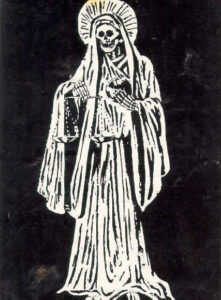
\includegraphics[scale=.5]{a20191027DeathandtheRealI-img001.jpg} 
\caption{Muerte Blanca} 
\end{wrapfigure}

I was driving on the highway at night, paying close attention to the traffic. A cop car ahead of me, a few cars in the lanes to my left. I accidentally turned off my headlights but could not turn them back on. Suddenly, the entire highway was pitch black. I continued to drive, unable to see anything ahead. The brakes did not work, yet the car was accelerating. I was weaving in and out, all the time thinking that I would crash into something. I speculated on what crash would occur while continuing to drive.

The ambiguity was clear. Was I heading into the darkness of death? Or was I being guided by unknown forces?

In Chapter V of \emph{Gnosis} Book 1, Boris Mouravieff includes a meditation on death, which comprised three exercises. The I of the Personality gives little thought to its own death. Mouravieff explains:

\begin{quotex}
All man can imagine in this respect is to evoke the image of his own corpse: he can never exclude from this representation the observer who contemplates this image. 

\end{quotex}

Only the Real I can contemplate one's death. While the ego looks for the light, the Real I faces the darkness. In most cases, it takes a major event, a boundary situations, to get the ego to face its own annihilation. Examples are: fright, guilt, finality, and suffering.

\begin{wrapfigure}{rt}{.3\textwidth}

\includegraphics[scale=.4]{a20191027DeathandtheRealI-img002.jpg} 
\end{wrapfigure}

\paragraph{Exercise 1: Remembrance of death}
\begin{quotex}
Death is the only real and unique event which happens to us without fail. In other words, constantly bearing in mind the idea of death approaching nearer every day is a concrete means of facing an implacable reality — before which all the joys and all the worries of the Personality fade. It is thus that one learns that in effect: `all is vanity and torments of the mind.' 

\end{quotex}
It is insufficient to read this exercise; rather, one must actually do it. The timing is good. During Halloween season in the USA, people decorate their lawns with images of death. Walk around the neighborhood and contemplate the skulls. It is better than candy.

This week: pray for the dead and visit a cemetery.

\paragraph{Exercise 2: The narrow road leading to Life}
\begin{quotex}
This is done by introducing a continuous and permanent attachment between the Personality and the passive Real `I'. so as to render the presence of the latter constant in the field of action of the Personality. Then, with time and according to the intensity of efforts, the situation can undergo a complete change: the more the Real I – like the grain of mustard seed – takes root in the mental life which was until then dominated by the Personality, the more the latter is subjected, little by little, to the will of the judge. Identifying himself with it, man will rediscover his Real `I' in all its integrity and permanence. For him, life then loses its factitious character, to become logical and factual. 

\end{quotex}
Train the ego, or false I, to become aware of the Real I. The ego lies to himself; it sugarcoats his life. The Real I judges rightly, which the ego dislikes. Ultimately, the goal is for the ego to become passive to the Real I. Learn to distinguish between the speech of the ego and the Real I.

\begin{quotex}
When a person speaks, it is generally easy to distinguish whether his records are playing or whether he speaks from some deeper part of himself. In the latter case, he uses a pictorial, rustic and sometimes awkward language; in the former he speaks in a singing tone of voice. 

\end{quotex}
\paragraph{Exercise 3: The philosopher's stone}
\begin{quotex}
The permanent link which must be introduced between the Personality and the real `I' is esoteric Knowledge. The knowledge and know-how that it permits us to acquire represent the philosophers' stone of the medieval mystics. They are capable of provoking in man the transmutation to which he aspires. 

\end{quotex}
Read the best material rather than wild speculations or useless opinions.

\paragraph{Summary:}
\begin{itemize}
\item Constantly bear in mind the idea of your own death 
\item Make the real I the master of the I of the Personality 
\item Acquire esoteric knowledge 
\end{itemize}
\paragraph{Leaving the I of the Personality Behind}
\begin{quotex}
the petty bourgeois is spiritless[.] … Devoid of imagination, as the petty bourgeois always is, he lives within a certain orbit of trivial experiences as to how things come about, what is possible, what usually happens, no matter whether he is a tapster or a prime minister. This is the way the petty bourgeois has lost himself and God. \flright{\textsc{Soren Kierkegaard}, \emph{The Sickness Unto Death}}

\end{quotex}


\flrightit{Posted on 2019-10-27 by Cologero }

\begin{center}* * *\end{center}

\begin{footnotesize}\begin{sffamily}



\texttt{Patricia on 2019-10-28 at 17:05 said: }

Your dream reminds me of the dark night of the senses that St. John of the Cross wrote about. The gift on the other side of that “night” erupts in the last sentence of your writing, concerning the moments when joy and beauty suddenly appear. I am so glad you made it through such a difficult medical and spiritual challenge.


\hfill

\texttt{Santiago on 2020-10-28 at 13:16 said: }

One of my favorite articles on the site. Steps 2 and 3 seem somewhat more difficult!

Regarding step 1, Evola states in Doctrine of Awakening, that it's a good practice to witness an autopsy and meditate on the nature of death. The idea being, if I recall correctly, to maintain an awareness that we are more than our physical body. There are many autopsies one may watch on YouTube, and all are quite grotesque, so squeamish viewers should overlook the provided example: https://www.nsfwyoutube.com/watch?v=nHeFUT-11So (NSFW)

“Only the Real I can contemplate one's death. While the ego looks for the light, the Real I faces the darkness. In most cases, it takes a major event, a boundary situations, to get the ego to face its own annihilation. Examples are: fright, guilt, finality, and suffering.”

Is the sensation of ego annihilation typically accompanied by a `deep' darkness and a profound, rapid sense of `falling'. I had this experience recently, and it was so overwhelming that I impulsively stood up and gasped for air, ending immediately the experience.


\hfill

\texttt{Greg on 2020-10-29 at 14:24 said: }

Is death the annihilation of the personality? If you listen to nde accounts it would seem not but I suppose they might be unreliable.


\end{sffamily}\end{footnotesize}
